% !TEX root = ../thesis.tex
% sensor-array prinziple
% @author Tobias Wulf
%

\section{Prinzip des Sensor-Arrays}\label{sec:prinzip-des-sensor-arrays}


Ein \gls{gl:sensor-array} stellt in seiner Funktionsweise ein Array aus einzelnen Winkelsensoren dar. Jeder einzelne Winkelsensor des Arrays bildet somit einen \gls{gl:sensor-pixel}. Die einzelnen Sensor-Pixel besitzen im Simulationsbetrieb das selbe Verhalten, das basierend auf den TMR-Senor \cite{TDK2016}, aus Kennfeldern (\autoref{ch:tdk-datensatz}) entnommen wird. Resultierende Messwerte der einzelnen Sensor-Pixel sind positionsabhängig von ihrer Lage im Sensor-Array\cite{Schuethe2019}. Die Sensor-Pixel-Anordnung erfolgt quadratisch mit gleichen Abständen zu einander. Das Gesamtsystem ist somit eine Adaption des klassischen Anwendungsfall aus \autoref{fig:klassischeranwendungsfall} für multiple Winkelsensoren \cite{Mehm2019}\cite{Schuethe2019}. So ergibt sich der Anwendungsfall für das Sensor-Array nach \autoref{fig:sensor-array-prinzip}.
\newline
Das Gesamtsystem aus Gebermagnet und Sensor-Array behält seinen Koordinatenursprung in der Gebermagnetmitte. Das Sensor-Array ist zentriert und lotrecht zur $Z$-Achse des Magneten auszurichten \cite{Schuethe2019}. Sodass ein konstantes Flächenniveau in $Z$ eingehalten wird. Bedingt durch die aufgespannte Array-Fläche, sind die einzelnen Sensor-Pixel nicht mehr ideal unter dem Magneten ausgerichtet \cite{Schuethe2020b}. Es ist somit davon auszugehen, dass die Kreisbahnen der einzelnen Pixel verzerrt sind. Wobei sich die Bahnbeschreibungen, der Pixel mit dem geringsten $X$-/ $Y$-Versatz, einem idealen Kreisverlauf annähern müssen. Physikalische Kleinstabstände zwischen den Sensorbrücken eines Sensor-Pixels sind vernachlässigt. Im Simulationsbetrieb ist die Annahme getroffen, dass die Brückenabstände innerhalb eines Sensor-Pixel vernachlässigbar klein sind.


\clearpage


\begin{figure}[tph]
	\centering
	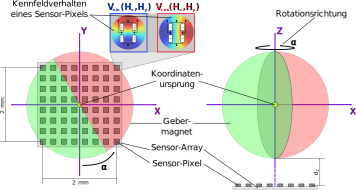
\includegraphics[width=.9\linewidth]{chapters/images/2-Grundlagen/Sensor-Array-Prinzip}
	\caption[Geometrischer Aufbau und Ausrichtung des Sensor-Arrays]{Geometrischer Aufbau und Ausrichtung des Sensor-Arrays. Quadratische Anordnung von Sensor-Pixeln zu einem $8 \times 8$ Sensor-Array. Alle Pixel sind gleich verteilt auf der Array-Fläche. Sensor-Pixel-Verhalten ist aus Kennfeldern entnommen und ortsabhängig von Pixel-Position im Koordinatensystem. Array-Kantenlängen sind mittig von Eck-Pixel zu Eck-Pixel bestimmt. Ebenfalls der $Z$-Abstand zur Magnetoberfläche. Abstände innerhalb der Pixel sind vernachlässigt. Das Array ist zentriert in der $Z$-Achse ausgerichtet. Ideal lotrecht zur Nord-Süd-Ausrichtung des Magneten. Koordinatenursprung des Gesamtsystem liegt in der Gebermagnetmitte. Gebermagnet ist ein Kugelmagnet, der um seine $Z$-Achse rotiert. Grafik nachempfunden und bearbeitet aus \cite{Schuethe2020b}.}
	\label{fig:sensor-array-prinzip}
\end{figure}


Gemäß der geometrischen Vorgaben, konstantem Flächenniveau in $Z$ und der Wahl des Koordinatenursprungs, fächert sich ein Koordinaten-Meshgrid für $N_{Pixel} \times N_{Pixel}$ für $i,j \in \{1 \ldots N_{Pixel} \}$ Sensor-Pixel auf. Dabei ist von einer, im Mittelpunkt des Sensor-Array festgelegten, Grundposition $\vec{p}$ des Sensor-Arrays nach \autoref{eq:arraymeshgrid} vorzugehen. 


\begin{alignat}{3}\label{eq:arraymeshgrid}
	&\vec{p} = \begin{pmatrix}p_x \\ p_y \\ p_z\end{pmatrix} \qquad && A_{Array} = a_{Array}^2 \qquad 					  && x_{i,j} = p_x - \frac{a_{Array}}{2} + j \cdot d_{Pixel} \nonumber\\
	& 																&& d_{Pixel} = \frac{a_{Array}}{N_{Pixel} - 1} \qquad && y_{i,j} = p_y + \frac{a_{Array}}{2} - i \cdot d_{Pixel} \\
	& 																&& 													  && z_{i,j} = p_z - r_{mag} = konst.\nonumber
\end{alignat}


Die  $Z$-Koordinate entspricht dem $Z$-Abstand zum Magneten mit $d_z = p_z$. Das Sensor-Array ist über diesen Vektor in Koordinatensystem zu verschieben. Der Koordinatenursprung bleibt im Magneten. Das Meshgrid fächert sich für die $i-te$ Reihe und die $j-te$ Spalte des Sensor-Arrays auf. Somit gibt jedes Sensor-Pixel, entsprechend seiner Zuordnung im Array, Spannungsausgaben wie ein einzelnes Sensor-IC aus. Es stehen dadurch nicht mehr Skalare bzw. ein Vektor als Winkelmesswert zur Verfügung, sondern Array-Daten für korrespondierende Cosinus- und Sinus-Vektorfelder \cite{Mehm2019}\cite{Schuethe2020}. \autoref{fig:sensor-array-daten} zeigt den dimensionalen Zuwachs. 


\vspace{5mm}
\begin{figure}[tph]
	\centering
	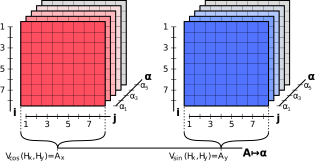
\includegraphics[width=0.9\linewidth]{chapters/images/2-Grundlagen/Sensor-Array-Daten}
	\caption[Resultierende Sensor-Array-Daten]{Resultierende Sensor-Array-Daten. Zwei Matrizen, je eine für alle Cosinus-Brückenausgaben und Sinus-Brückenausgaben. Die $i-ten$ und $j-ten$ Matrixelemente bilden eine Vektor entsprechend des klassischen Anwendungsbeispiels. Jeweils ein Matrix-Paar für die $n-te$ Winkelstellung $\alpha$.}
	\label{fig:sensor-array-daten}
\end{figure}


Bedingt durch den Zuwachs an Daten und ihre Anordnung, benötigt es eine modifizierte Abstandsfunktion \cite{Schuethe2020b}\cite{Schuethe2020} im Vergleich zur \autoref{eq:de2innorm}. Als erstes braucht es skalare Repräsentanten der Matrizen. Diese sind durch eine zutreffende Matrix-Norm zu bilden. Matrizen können als lange Vektoren betrachtet werden, daher bietet sich die Rechenvorschrift für $j-te$ Spalten nach \autoref{eq:fnorm} an. Diese Norm ist als Frobenius-Norm bezeichnet.


\begin{equation}\label{eq:fnorm}
\|\mathbf{A_x}\|_F= \sqrt{\sum_{j=1}^{n}\|A_{xj}\|_2^2} = \sqrt{\mathbf{A_x}\mathbf{A_x}^T}
\end{equation}


\clearpage


Angewandt auf beide Vektormatrizen für Cosinus- und Sinus-Anteile, ergibt sich eine normierte Kreisbahn nach \autoref{eq:rinfnorm}. Der Radius ist durch Versatz der einzelnen Sensor-Pixel nicht konstant und muss je nach Position des Sensor-Arrays eine weniger oder stärkere Ellipsenform beschreiben \cite{Schuethe2019}. Das ergibt sich durch Überlagerung der Sinoiden nach Frobenius-Norm. Der Versatz jedes einzelnen Sensor-Pixel wirkt dabei wie eine Dämpfung auf die Ausgangsspannungen der Sensor-Pixel. So zeigt sich ein Versatz in $X$-Richtung in einer Dämpfung der Cosinus-Funktion und entsprechender Versatz in $Y$-Richtung mit einer Dämpfung der Sinus-Funktion \cite{Schuethe2019}.


\begin{equation}\label{eq:rinfnorm}
	\|r\|_F = \big|\|\mathbf{A}\|_F\big| = \sqrt{\|\mathbf{A_x}\|_F^2 + \|\mathbf{A_y}\|_F^2}
\end{equation}


Durch simples einsetzen der normierten Messwertmatrizen in die euklidische Abstandsquadratfunktion \autoref{eq:de2innorm}, folgt ein approximiertes Abstandsergebnis nach \autoref{eq:fnorminde2}. Über die Dreiecksungleichung erhält man die genau Lösung und Projektion in den höheren Normraum \cite{Plum2012}\cite{vandeGeijn2014} und somit die modifizierte Abstandsfunktion nach Frobenius-Norm \cite{Schuethe2020}\cite{Schuethe2020b} in \autoref{eq:df2}. Es sind gemachte Beschreibungen aus \autoref{sec:euklidischer-abstand}, für zwei Winkelstellungen $\mathbf{A}$ und $\mathbf{B}$, entsprechend der Array-Datenformate angepasst.


\begin{align}
\label{eq:fnorminde2}
d_E^2\langle\mathbf{A},\mathbf{B}\rangle &= \big(\|\mathbf{A_x}\|_F - \|\mathbf{B_x}\|_F\big)^2 + \big(\|\mathbf{A_y}\|_F - \|\mathbf{B_y}\|_F\big)^2 \\
&\le \nonumber \\
\label{eq:df2}
d_F^2\langle\mathbf{A},\mathbf{B}\rangle &= \|\mathbf{A_x} - \mathbf{B_x}\|_F^2 + \|\mathbf{A_y} - \mathbf{B_y}\|_F^2 = \|\mathbf{A} - \mathbf{B}\|_F^2
\end{align}


